\documentclass[UTF8,aspectratio=169,presentation]{ctexbeamer}
\usetheme{Madrid}

\usefonttheme{serif}              % 使用衬线字体
\usefonttheme{professionalfonts}  % 数学公式字体
\usepackage{zhnumber}
\usepackage{soul}
\usepackage{amsmath}
\usepackage{hyperref}
\usepackage[overload]{empheq}
\usepackage{tikz}

% Change base colour beamer@blendedblue (originally RGB: 0.2,0.2,0.7)
\colorlet{beamer@blendedblue}{green!40!black}

\titlegraphic{
    
\includegraphics[width=2cm]{images/bit.png}
}


\usepackage{xspace}

\makeatletter
\let\HL\hl
\renewcommand\hl{%
  \let\set@color\beamerorig@set@color
  \let\reset@color\beamerorig@reset@color
  \HL}
\makeatother

\newtheorem{assumption}{Assumption}
\newtheorem{remark}{Remark}
\newtheorem{mytheorem}{Theorem}

\usepackage{color}
\usepackage[ruled,lined,noend]{algorithm2e}
\usepackage{fontspec}
\setmainfont{Liberation Serif}
%\setsansfont{DejaVu Sans}
%\setmonofont{Cousine}
\usepackage{xeCJK}
%\setCJKmainfont[BoldFont=Noto Sans SC]{Noto Serif SC}
\setCJKsansfont{Noto Sans SC}
\setCJKmonofont{WenQuanYi Micro Hei Mono}


\usetheme{default}
%\usecolortheme{orchid}

\parindent2em


\begin{document}

%% --> 导言页
\title{NIPS-2017 Federated Multi-Task Learning}
\author{冯开宇}
\institute{北京理工大学}
\date{\zhtoday}
\frame{\titlepage}



\addtobeamertemplate{frametitle}{}{%
\begin{tikzpicture}[remember picture,overlay]
\node[anchor=north east,yshift=2pt] at (current page.north east) {
\includegraphics[height=0.8cm]{images/bit.png}};
\end{tikzpicture}}

%% --> 目录结构
%
\begin{frame}{目录}
  \tableofcontents[hideallsubsections]
\end{frame}

%% --> 正式内容开始
%
\section{Summary}    % 第 1 节

%% 每一节开头显示目录,并高亮当前节的主题
\AtBeginSection[]{\frame{\tableofcontents[currentsection,hideallsubsections]}}

%% --> 第 1 帧
\begin{frame}{Summary}{TL;DR}

  In this work, we show that \hl{multi-task learning is naturally suited to handle the statistical challenges of this setting (federated learning)}, and propose a novel systems-aware optimization method, \hl{MOCHA (which generalizes the distributed optimization method COCOA), that is robust to practical systems issues.}

\end{frame}

\section{What is federated learning}    % 第 2 节

\newcommand{\eg}{e.g.\@\xspace}

%% --> 第 2 帧
\begin{frame}{What is Federated Learning}{the Motivating of Federated Learning}
\begin{columns}[T] % align columns
\begin{column}{.48\textwidth}
\color{red}
\eg (1)
\rule{\linewidth}{4pt}
\color{black}


\textbf{Problem}: Google want to train model with users' mobile data.

\textbf{Possible solution} Centralized learning.

\textbf{Challenge} \eg GDPR.


\end{column}%
\hfill%
\begin{column}{.48\textwidth}
\color{blue}
\eg (2)
\rule{\linewidth}{4pt}
\color{black}

\textbf{Problem}: Several hospitals want to jointly train a better model use medical data.

\textbf{Possible solution} Centralized learning (through aggregated data).

\textbf{Challenge} Laws or policies may forbid giving patients' data to others.
\end{column}%
\end{columns}


\end{frame}


\begin{frame}
  \frametitle{What is Federated Learning}
  \framesubtitle{Federated Learning vs. Distributed Learning}
  \begin{center}
    \underline{Federated learning is one of the distributed learning.}
  \end{center}
  \vspace{0.5cm}

Main differences are:
\begin{itemize}
  \item Users have control over their device and data.
  \item Worker nodes are unstable.
  \item \textbf{Communication cost is higher than computation cost}
  \item Data stored on worker nodes are \textbf{not IID}.
  \item The amount of data is severely imbalanced.
\end{itemize}



Which lead to ...

\end{frame}

\begin{frame}
  \frametitle{What is Federated Learning}
  \framesubtitle{Consideration (Research Direction) in Federated Learning System Design}

\begin{itemize}
  \item \textit{Trade Computation for Communication} \footnote{mainly focused in this paper.}
  \item Privacy
  \item \textit{Robustness} \footnotemark[\value{footnote}]
\end{itemize}

\vspace{1cm}


\end{frame}


\begin{frame}[t]
  \frametitle{What is Federated Learning}
  \framesubtitle{Related Work: Multi-task Learning}
  \hl{In multi-task learning, the goal is to learn models for multiple related tasks simultaneously.}

    While the MTL literature is extensive, most MTL modeling approaches can be broadly categorized into two groups based on how they capture relationships amongst tasks. The first assumes that a clustered, sparse, or low-rank structure between the tasks is known a priori. \ul{ A second group instead assumes that the task relationships are not known beforehand and can be learned directly from the data. }

    \hl{In comparison to learning a single global model, these MTL approaches can directly capture relationships amongst non-IID and unbalanced data}, which makes them particularly well-suited for the statistical challenges of federated learning.
  
\end{frame}


 \section{MOCHA - Model}

\begin{frame}[t]
  \frametitle{MOCHA - Model}
  \framesubtitle{The Problem We are Facing}

\begin{itemize}
  \item \textbf{Statistical Challenges}: The aim in federated learning is to fit a model to data,$\left\{\mathbf{X}_{1}, \ldots, \mathbf{X}_{m}\right\}$, generated by $m$ distributed nodes. \hl{Each node, $t \in[m]$, collects data in a \textit{non-IID} manner across the network}, with data on each node being generated by a distinct distribution $\mathbf{X}_{t} \sim P_{t}$. \hl{The number of data points on each node,$n_t$ , may also vary significantly}, and there may be an underlying structure present that captures the relationship amongst nodes and their associated distributions.
  \sethlcolor{cyan}
\item \textbf{Systems  Challenges}:  There are typically a large number of nodes, $m$,  in the network,  and \hl{communication is often a significant bottleneck}. Additionally, the storage, computational, and communication capacities of each node may differ due to variability in hardware (CPU, memory), network connection (3G, 4G, WiFi), and power (battery level). \hl{These systems challenges, compounded with unbalanced data and statistical heterogeneity, make issues such as stragglers and fault tolerance significantly more prevalent than in typical data center environments.}
\end{itemize}
\end{frame}


\newcommand{\eqone}{
   \min _{\mathbf{W}, \boldsymbol\Omega}\left\{\sum_{t=1}^{m} \sum_{i=1}^{n_{t}} \ell_{t}\left(\mathbf{w}_{t}^{T} \mathbf{x}_{t}^{i}, y_{t}^{i}\right)+\mathcal{R}(\mathbf{W}, \boldsymbol{\Omega})\right\}
}

 \begin{frame}[t]
   \frametitle{MOCHA - Model}
   \framesubtitle{General Multi-Task Learning Setup}

   Given data $\mathbf X_t  \in \mathbb R^{d×n_t}$ from $m$ nodes ($t \in [m]$), multi-task learning fits separate weight vectors $\mathbf w_t \in \mathbb R^d$ to
   the data for each task (node) through arbitrary \hl{convex loss functions $\ell^t$} (e.g., the hinge loss for SVM models). Many MTL problems can be captured via the following general formulation:
   $$
   \eqone
  $$
  As an example, several popular MTL approaches assume that tasks form clusters based on whether or not they are related. This can be expressed via the following \hl{bi-convex} formulation:

$$
\mathcal{R}(\mathbf{W}, \boldsymbol{\Omega})=\lambda_{1} \operatorname{tr}\left(\mathbf{W} \boldsymbol{\Omega}\mathbf{W}^{T}\right)+\lambda_{2}\|\mathbf{W}\|_{F}^{2}
$$
  
With constants $\lambda_1,\lambda_2 >0$, and where the second term performs $L_2$ regularization on each local model.

 \end{frame}
\begin{frame}[t]
  \frametitle{MOCHA - Model}
  \framesubtitle{Algorithm}

  \small
  \begin{algorithm}[H]
  \caption{MOCHA: Federated Multi-Task Learning Framework}\label{algorithm}
  \KwIn{Data $\mathbf{X}_t$ from $t = 1, ..., m $ tasks, stored on one of $m$ nodes, and initial matrix $\boldsymbol{\Omega}_0$}
  Starting point $\boldsymbol{ \alpha }^{(0)} := 0 \in \mathbb{R}^n, \mathbf{ v }^{(0)} := 0 \in \mathbb{R}^b$

  \For{\textbf{iterations}$i = 0, 1, ...$}{

    Set subproblem parameter $\sigma^{\prime}$ and number of federated iterations, $H_i$

    \For{\textbf{iterations} $h = 0,1, ..., H_i$ }{

      \For{\textbf{tasks $t \in \{1, 2, ..., m\} $ in parallel over $m$ nodes }}{
        \hl{call local solver, returning $\theta_t^h$-approximate solution $\Delta\boldsymbol{ \alpha }_t$ of the local subproblem}

        update local variables $\boldsymbol{\alpha}_t \leftarrow \boldsymbol{\alpha}_t + \Delta\boldsymbol{\alpha}_t$

        return updates $\Delta \mathbf{v}_t := \mathbf{X}_t \Delta\boldsymbol{\alpha}_t$
      }
      \textbf{Reduce:} $\mathbf v_t \leftarrow \mathbf v_t + \Delta \mathbf v_t$
    }
    Update $\boldsymbol{\Omega}$ centrally based on $\mathbf{w}(\boldsymbol\alpha)$ for latest $\boldsymbol{ \alpha }$
  }
  Centrol node computes $\mathbf{w}= \mathbf{w}(\boldsymbol{\alpha})$ based on the latest $\boldsymbol{\alpha}$

  \KwRet{$\mathbf{ W } := [\mathbf w_1, ..., \mathbf w_m]$}
  \end{algorithm}
\end{frame}

  \begin{frame}[t]
    \frametitle{MOCHA - Model}
    \framesubtitle{About $\boldsymbol\Omega$}
    \begin{itemize}
      \item \textbf{ Observation 1: } In general, (1) is not jointly convex in $\mathbf W$ and $\boldsymbol\Omega$, and even in the cases where (1) is convex, solving for $\mathbf W$ and $\boldsymbol\Omega$ simultaneously can be difficult.
     \item \textbf{ Observation 2: } When fixing $\boldsymbol\Omega$, updating $\mathbf W$ depends on both the data $\mathbf X$, which is distributed across the nodes, and the structure $\boldsymbol \Omega$, which is known centrally.
    \item \textbf{ Observation 3: } When fixing $\mathbf W$, optimizing for $\boldsymbol\Omega$ only depends on $\mathbf W$ and not on the data $\mathbf X$.
  \end{itemize}
  
\end{frame}

  \newcommand{\eqtwo}{
  \min _{\boldsymbol\alpha}\left\{\mathcal{D}(\boldsymbol{\alpha}):=\sum_{t=1}^{m} \sum_{i=1}^{n_{t}} \ell_{t}^{*}\left(-\boldsymbol{\alpha}_{t}^{i}\right)+\mathcal{R}^{*}(\mathbf{X} \boldsymbol{\alpha})\right\}
  }
\begin{frame}[t]{MOCHA - Model}{Dual Problem}

  Let $n:=\Sigma^m_{t=1} n_t $ and $X := Diag(X_1,···,X_m) \in \mathbb{R}^{md\times n}$.  With $\boldsymbol\Omega$ fixed, the dual of problem(1), defined with respect to dual variables $\boldsymbol\alpha \in \mathbb R^n$, is given by:

  $$
  \eqtwo
  $$

  where $\ell^*_t$ and $\mathcal R^*$ are the conjugate dual functions of $\ell_t$ and $\mathcal{R}$, respectively, and $\boldsymbol\alpha^i_t$ is the dual variable for the data point $(x^i_t,y^i_t)$.
\end{frame}

\begin{frame}[t]
\begin{assumption}[1]
  Given $\boldsymbol\Omega$, we assume that there exists a symmetric positive definite matrix $\mathbf M \in \mathbb R^{md×md}$, depending on $\boldsymbol\Omega$, for which the function $\mathcal R$ is strongly convex with respect to $\mathbf M^{−1}$ . Note
  that this corresponds to \hl{assuming that $\mathcal R^{*}$ will be smooth with respect to matrix $\mathbf M$}.
  
\end{assumption}

\begin{remark}[1]
  We can reformulate the MTL regularizer in the form of $\bar{\mathcal R}(\mathbf w, \bar{\boldsymbol\Omega}) = \mathcal R( \mathbf W, \boldsymbol\Omega$), where
  $\mathbf w \in \mathbb R^{md}$ is a vector containing the columns of $\mathbf W$ and $ \bar{\boldsymbol \Omega}  := \boldsymbol\Omega \otimes \mathbf I_{d×d} \in \mathbb R^{md\times md}$
  . For example, we can rewrite the regularizer in (2) as $\bar{\mathcal R}( \mathbf w,\bar{\boldsymbol \Omega} ) = tr(\mathbf w^T (\lambda_1 \bar{\boldsymbol\Omega}+ \lambda_2 \mathbf I) \mathbf w)$. Writing the regularizer
  in this form, it is clear that it is strongly convex with respect to matrix $\mathbf M^{−1} = \lambda_1 \bar{\boldsymbol\Omega}+ \lambda_2 \mathbf I$.
\end{remark}
\end{frame}


\begin{frame}[c]


CoCoA (Fenchel-Rockafellar
duality):

\begin{subequations}
  \begin{align}[left=\empheqlbrace]
      & \min _{\boldsymbol{\alpha} \in \mathbb{R}^{n}}  \left\{ {\mathcal{O}_{A}(\boldsymbol{\alpha}) :=f(A \boldsymbol{\alpha})+g(\boldsymbol{\alpha})} \right\} , \label{eq:a1} \\
      & \min _{\mathbf{w} \in \mathbb{R}^{m}} {\left\{\mathcal{O}_{B}(\mathbf{w}) :=f^{*}(\mathbf{w})+g^{*}(-A^{\top} \mathbf{w})\right\}},  \label{eq:a2}
    \end{align}
\end{subequations}

MOCHA:

\begin{subequations}
  \begin{align}[left=\empheqlbrace]
      & \eqone, \label{eq:b1} \\
      & \eqtwo, \label{eq:b2} 
    \end{align}
\end{subequations}

\ref{eq:a1} matches \ref{eq:b2}, and \ref{eq:a2} matches \ref{eq:b1}. $\ell_t$ matches $g$ and vice versa.

\end{frame}

\begin{frame}[t]
  \frametitle{MOCHA}
  \framesubtitle{Data-local quadratic subproblems}

  The following
  data-local subproblems is a careful quadratic approximation of the dual problem to separate computation across the nodes. These subproblems find updates $\Delta \boldsymbol \alpha _t \in \mathbb R^{n_t}$ to the dual
  variables in $\boldsymbol\alpha$ corresponding to a single node $t$, and only require accessing data which is available locally, i.e., $\mathbf X_t$ for node $t$. The $t$-th subproblem is given by:
  \begin{align*}
    \min _{\Delta \alpha_{t}} \mathcal{G}_{t}^{\sigma^{\prime}}\left(\Delta \boldsymbol{\alpha}_{t} ; \mathbf{v}_{t}, \boldsymbol{\alpha}_{t}\right) &:=\sum_{i=1}^{n_{t}} \ell_{t}^{*}\left(-\boldsymbol{\alpha}_{t}^{i}-\Delta \boldsymbol{\alpha}_{t}^{i}\right) \\
  & +\left\langle\mathbf{w}_{t}(\boldsymbol{\alpha}), \mathbf{X}_{t} \Delta \boldsymbol{\alpha}_{t}\right\rangle+\frac{\sigma^{\prime}}{2}\left\|\mathbf{X}_{t} \Delta \boldsymbol{\alpha}_{t}\right\|_{\mathbf{M}_{t}}^{2}+c(\boldsymbol{\alpha}),
  \end{align*}
  where $c(\boldsymbol\alpha) := \frac{1}{m} \mathcal R^{*}({\mathbf X \boldsymbol \alpha})$, and $\mathbf M_t \in \mathbb R^{d \times d}$ is the $t$-th diagonal block of the symmetric positive definite matrix $\mathbf M$.

  Given dual variables $\boldsymbol\alpha$, corresponding primal variables can be found via $\mathbf w (\boldsymbol \alpha) = \nabla {\mathcal{R}^{*}} (\mathbf X \boldsymbol\alpha) $, where $\mathbf w_t(\boldsymbol\alpha)$ is the $t$-th block in the vector $\mathbf{w}(\boldsymbol\alpha)$.


\end{frame}

\begin{frame}[t]

  \begin{align*}
    \min _{\Delta \alpha_{t}} \mathcal{G}_{t}^{\sigma^{\prime}}\left(\Delta \boldsymbol{\alpha}_{t} ; \mathbf{v}_{t}, \boldsymbol{\alpha}_{t}\right) &:=\sum_{i=1}^{n_{t}} \ell_{t}^{*}\left(-\boldsymbol{\alpha}_{t}^{i}-\Delta \boldsymbol{\alpha}_{t}^{i}\right) \\
  & +\left\langle\mathbf{w}_{t}(\boldsymbol{\alpha}), \mathbf{X}_{t} \Delta \boldsymbol{\alpha}_{t}\right\rangle+\frac{\sigma^{\prime}}{2}\left\|\mathbf{X}_{t} \Delta \boldsymbol{\alpha}_{t}\right\|_{\mathbf{M}_{t}}^{2}+c(\boldsymbol{\alpha}),
  \end{align*}

Note that computing $\mathbf{w}(\boldsymbol\alpha)$ requires 
  the vector $\mathbf v = \mathbf X \boldsymbol \alpha$. \hl{The $t$-th block of $\mathbf v, \mathbf v_t \in \mathbb R^d$ , is the only information that must be communicated
between nodes at each iteration.}

One interesting aspect of MOCHA is that \hl{the method can be easily modified to accommodate the
sharing of tasks among the nodes without any change to the local solvers}. This property helps the
central node to reduce the size of $\boldsymbol\Omega$ and the complexity of its update with minimal changes to the
whole system.
\end{frame}

\section{MOCHA - Convergence Analysis}

\begin{frame}[t]
  \frametitle{Convergence Analysis}
  \framesubtitle{Approximately solvable subproblem}
  We define $\theta_t^h$ as a function of these factors, and assume that each node has a controller that may derive $\theta_t^h$ from the current clock cycle and statistical/systems setting. $\theta_t^h$ ranges from zero to one, where $\theta^h_t = 0$ indicates an exact solution to $\mathcal G^{\sigma^{\prime}}_t(·)$and $\theta^h_t= 1$ indicates that node $t$ made no progress during iteration $h$ (which we refer to as a \textit{dropped node}).
  $$
\theta_{t}^{h}:=\frac{\mathcal{G}_{t}^{\sigma^{\prime}}\left(\Delta \boldsymbol{\alpha}_{t}^{(h)} ; \mathbf{v}^{(h)}, \boldsymbol{\alpha}_{t}^{(h)}\right)-\mathcal{G}_{t}^{\sigma^{\prime}}\left(\Delta \boldsymbol{\alpha}_{t}^{\star} ; \mathbf{v}^{(h)}, \boldsymbol{\alpha}_{t}^{(h)}\right)}{\mathcal{G}_{t}^{\sigma^{\prime}}\left(\mathbf{0} ; \mathbf{v}^{(h)}, \boldsymbol{\alpha}_{t}^{(h)}\right)-\mathcal{G}_{t}^{\sigma^{\prime}}\left(\Delta \boldsymbol{\alpha}_{t}^{\star} ; \mathbf{v}^{(h)}, \boldsymbol{\alpha}_{t}^{(h)}\right)}
$$
where $\Delta \boldsymbol\alpha^{*}_t$ is the minimizer of subproblem $\mathcal G_t^{\sigma}(· ; \mathbf v^{(h)} ,\boldsymbol\alpha^t )$.

\end{frame}


\begin{frame}
  \begin{assumption}[2]
  Let $\mathcal H_h := (\boldsymbol\alpha^{(h)},\boldsymbol\alpha^{(h−1)},···,\boldsymbol\alpha^{(1)})$ be the dual vector history until the beginning of iteration $h$, and define $\Theta^h_t := \mathbb E[\theta^h_t|\mathcal H_h]$.  For all tasks $t$ and all iterations $h$, we assume $p^h_t:=\mathcal P[\theta^h_t= 1] \leq p_{max} < 1  \; and  \;  \hat{\Theta}^h_t:= \mathbb E[\theta^h_t| \mathcal H_h,\theta^h_t< 1] \leq \theta_{max} < 1$.
\end{assumption}

This assumption states that at each iteration, the probability of a node sending a result is non-zero, and that the quality of the returned result is, on average, better than the previous iterate.
\end{frame}

%\newtheorem{theorem}{Theorem}

\begin{frame}[t]
  \frametitle{MOCHA - Convergence Analysis}
  \framesubtitle{Convergence}

  \begin{mytheorem}[1]
    
    Assume that the losses $\ell_t$ are \hl{$(1/\mu)-smooth$}. Then, under Assumptions 1 and 2, there
    exists a constant $s \in (0, 1]$ such that for any given convergence target $\epsilon_{\mathcal D}$ , choosing $H$ such that

$$
H \geq \frac{1}{(1-\bar{\Theta}) s} \log \frac{n}{\epsilon_{\mathcal{D}}}
$$

will satisfy $
\mathbb{E}\left[\mathcal{D}\left(\boldsymbol{\alpha}^{(H)}\right)-\mathcal{D}\left(\boldsymbol{\alpha}^{\star}\right)\right] \leq \epsilon_{\mathcal{D}}
$.
  \end{mytheorem}

  Here, $\bar\Theta := p_{max} + (1 − p_{max} ) \Theta_{max} < 1$. While Theorem 1 is concerned with finite horizon convergence, it is possible to get asymptotic convergence results, i.e., $H \rightarrow \infty$, with milder assumptions on
the stragglers; see Corollary 8 in the Appendix for details.
\end{frame}

\begin{frame}[t]
  \frametitle{Convergence Analysis}
When the loss functions are non-smooth, e.g., the hinge loss for SVM models, we provide the
following sub-linear convergence for L-Lipschitz losses.

\begin{mytheorem}[2]
  If the loss functions $\ell_t$ are \hl{L-Lipschitz}, then there exists a constant $\sigma$, defined in (24),
  such that for any given $\epsilon_{\mathcal D} > 0$, if we choose

$$
\begin{array}{c}
H \geq H_{0}+\left[\frac{2}{(1-\bar{\Theta})} \max \left(1, \frac{2 L^{2} \sigma \sigma^{\prime}}{n^{2} \epsilon_{\mathcal{D}}}\right)\right] \\
\text { with } H_{0} \geq\left[h_{0}+\frac{16 L^{2} \sigma \sigma^{\prime}}{(1-\bar{\Theta}) n^{2} \epsilon_{\mathcal{D}}}\right], h_{0}=\left[1+\frac{1}{(1-\bar{\Theta})} \log \left(\frac{2 n^{2}\left(D\left(\boldsymbol{\alpha}^{\star}\right)-D\left(\boldsymbol{\alpha}^{0}\right)\right)}{4 L^{2} \sigma \sigma^{\prime}}\right)\right]_{+}
\end{array}
$$

then $
\overline{\boldsymbol{\alpha}}:=\frac{1}{H-H 0} \sum_{h=H_{0}+1}^{H} \boldsymbol{\alpha}^{(h)}
$ will satisfy $
\mathbb{E}\left[\mathcal{D}(\overline{\boldsymbol{\alpha}})-\mathcal{D}\left(\boldsymbol{\alpha}^{\star}\right)\right] \leq \epsilon_{\mathcal{D}}
$.
  
\end{mytheorem}


  
\end{frame}

\begin{frame}[t]
  \frametitle{Simulation}
  \framesubtitle{Datasets}

\begin{itemize}
  \item \textbf{Google Glass (GLEAM):} This dataset consists of two hours of high resolution sensor datacollected from 38 participants wearing Google Glass for the purpose of activity recognition.Following [41], we featurize the raw accelerometer, gyroscope, and magnetometer data into \textbf{180 statistical, spectral, and temporal features}.  We \textbf{model each participant as a separate task, and predict between eating and other activities} (e.g., walking, talking, drinking).
  \item \textbf{Human Activity Recognition:} Mobile phone accelerometer and gyroscope data collected from \textbf{30 individuals}, \textbf{performing one of six activities}: {walking, walking-upstairs, walking-downstairs,sitting,  standing,  lying-down}.   We  use  the  provided  561-length  feature  vectors  of  time  andfrequency domain variables generated for each instance.  We \textbf{model each individual as a separate task and predict between sitting and the other activities}.
\end{itemize}
\end{frame}

\begin{frame}[t]
  \begin{itemize}
    \item \textbf{Vehicle Sensor:} Acoustic, seismic, and infrared sensor data collected from a distributed network of 23 sensors, deployed with the aim of classifying vehicles driving by a segment of road. Each instance is described by \textbf{50 acoustic and 50 seismic features}.  We \textbf{model each sensor as aseparate task and predict between AAV-type and DW-type vehicles}.
  \end{itemize}
  
\end{frame}

\renewcommand{\figurename}{Figure}

\begin{frame}[t]
  \frametitle{Simulation}
  \framesubtitle{Multi-Task v.s. Global}
  \begin{figure}[htpb]
    \centering
    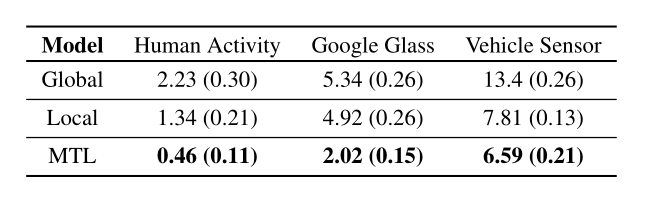
\includegraphics[width=0.8\linewidth]{images/mtl-result.png}
    \caption{Average prediction error: Means and standard errors over 10 random shuffles.}%
    \label{fig:1}
  \end{figure}

\end{frame}

\begin{frame}[t]
  \frametitle{Simulation}
  \framesubtitle{Statistical Heterogeneity a.k.a. Straggler Avoidance}
  % figure
  \begin{figure}[htpb]
    \centering
    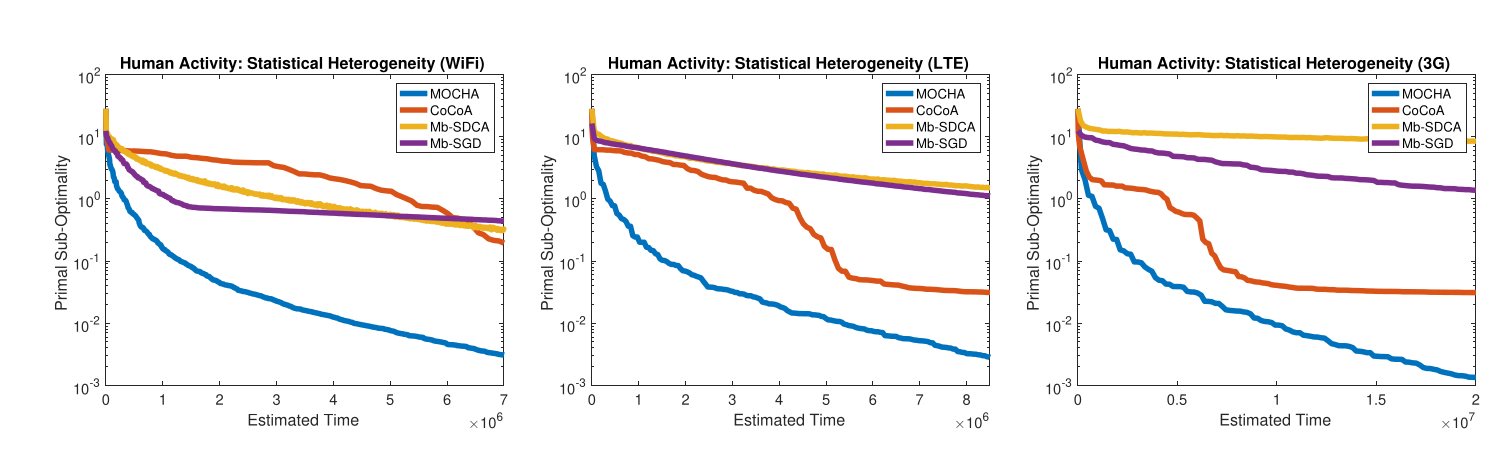
\includegraphics[width=0.8\linewidth]{images/statistical.png}
    \caption{The performance of MOCHA compared to other distributed methods for the $\mathbf W$ update of equation in MTL settings. While
increasing communication tends to decrease the performance of the mini-batch methods, MOCHA performs well
in high communication settings. In all settings, MOCHA with varied approximation values, $Θ^h_t$ , performs better than without (i.e., naively generalizing COCOA), as it avoids stragglers from statistical heterogeneity.}%
    \label{fig:2}
  \end{figure}
\end{frame}

\begin{frame}[t]
  \frametitle{Simulation}
  \framesubtitle{Systems Heterogeneity a.k.a. Data Variability}
  \begin{figure}[htpb]
    \centering
    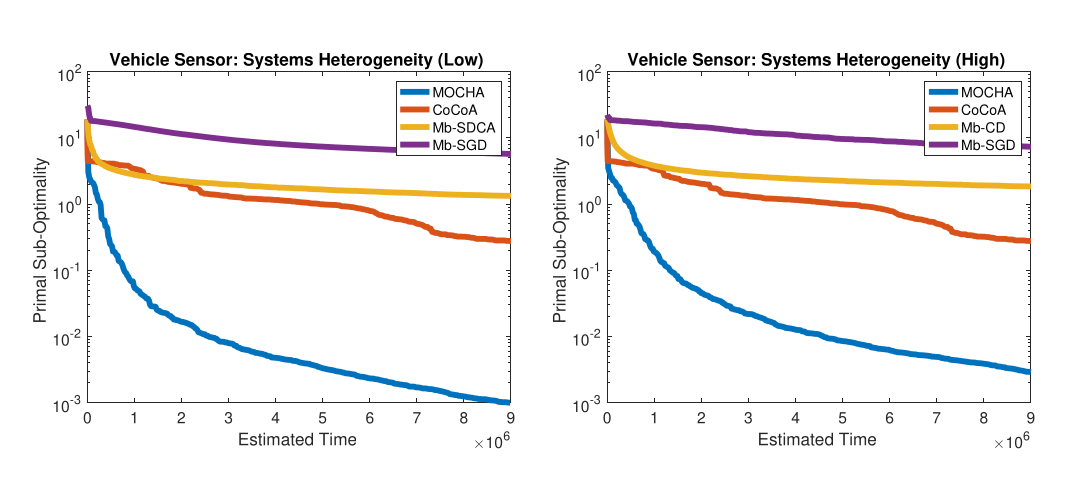
\includegraphics[width=0.8\linewidth]{images/system.png}
    \caption{MOCHA can handle variability from systems heterogeneity.}%
    \label{fig:name}
  \end{figure} 
\end{frame}


\begin{frame}[t]
  \frametitle{Simulation}
  \framesubtitle{Tolerance to Dropped Nodes}
  \begin{figure}[htpb]
    \centering
    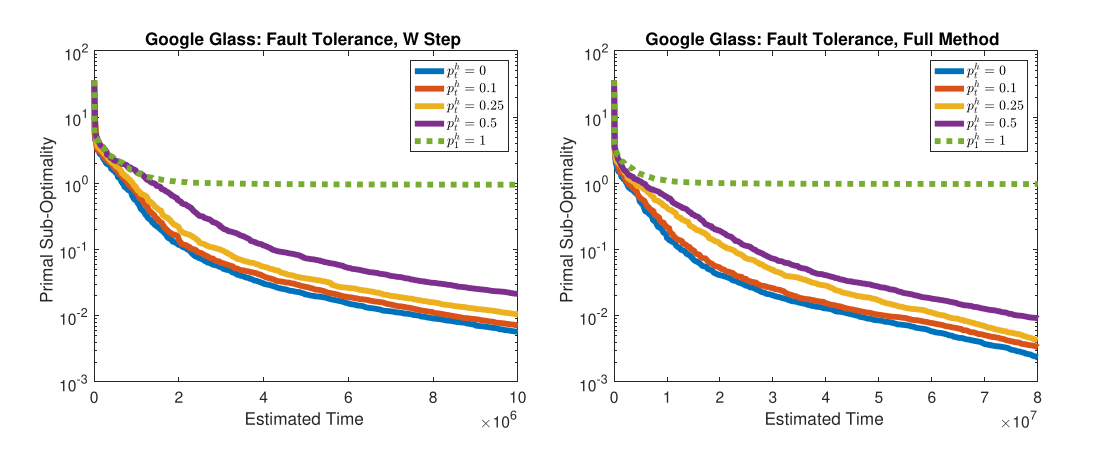
\includegraphics[width=0.8\linewidth]{images/2021-05-27_13-15.png}
    \caption{The performance of MOCHA is robust to nodes periodically dropping out (fault tolerance).}%
    \label{fig:4}
  \end{figure} 
\end{frame}

\section{Discussion}

\begin{frame}[t]
  \frametitle{Discussion}
  \framesubtitle{in the Paper}

  While MOCHA \hl{does not apply to non-convex deep learning models} in its current form, we note that there may be natural
connections between this approach and “convexified” deep learning models in the
context of kernelized federated multi-task learning.
  
\end{frame}


\begin{frame}[t]
  \frametitle{Discussion}
  \framesubtitle{Revierwer}

  \begin{itemize}
  \item The only major suggestion I would give is to possibly include discussion (or future work) \hl{addressing the limitation of requiring convex loss in real applications}, \hl{how techniques presented in this work may benefit distributed nonconvex problems}, and/or \hl{how they may benefit from "convexified" stronger models} (e.g. [1-4]).
  \item Not very novel (compared to COCOA) and \hl{just a mild variation over COCOA including the analysis}.
  \item After the author feedback, it became clear that the synchronous updates and the changes to CoCoa have merit. \hl{Most of the intellectual contribution is on the convergence analysis rather than the learning algorithm, which is both a strong and a weak point.}

  \end{itemize}

[1] Convex Deep Learning via Normalized Kernels, NIPS 2014

[2] Convolutional Kernel Networks, NIPS 2014

[3] Tensor Switching Networks, NIPS 2016

[4] Convexified Convolutional Neural Networks, ICML 2017
\end{frame}

\begin{frame}[c]

  Thanks!
  
\end{frame}

\end{document}
